%----------------------------------------------------------------------
%	CERN TEST BEAM CHAPTER
%----------------------------------------------------------------------
\label{ch:analysis}

Along with determining the focal plane and radiation hardness of the 3-layer lens design, another crucial step towards solidifying an EIC DIRC design was to test the new lens in a prototype DIRC with a real particle beam. Because not all of the components of the high-performance DIRC baseline design for an EIC are currently available it is necessary to validate the simulation package currently used to design and optimize the system. In June and July of 2015 the PANDA Barrel DIRC group along with myself and Dr. Grzegorz Kalicy from CUA conducted a test beam at the European Organization for Nuclear Research (CERN) with a prototype DIRC for the PANDA experiment. This was used as an opportunity to evaluate the performance of the 3-layer lens in a real particle beam. The beam was a hadron-rich beam with momentum tunable from 1 - 10 GeV/c. A standalone GEANT4 simulation package developed for the PANDA DIRC prototype (and later modified for the EIC DIRC geometry) was used for look-up table (LUT) generation, data monitoring, and comparison to data.
%The EIC DIRC simulation package was modified to use this new geometry setup so that data could be compared to simulation. 
The two most important quantities measured during this test beam were the photon yield per track and the Single Photon Resolution (SPR). Verifying these measurements with simulation give a good indication that the performance shown in Chapter \ref{ch:eicdirc} is what should be reasonably expected from a real EIC DIRC detector.

%----------------------------------------------------------------------
%	PROTOTYPE SETUP SECTION
%----------------------------------------------------------------------
\section{2015 Test Beam Prototype Setup}
The PANDA prototype was situated in the CERN Proton Synchrotron (PS) T9 experimental hall \cite{CERN_T9}. A 200 mm thick aluminum target upstream of the T9 hall was used to produce a hadron-rich beam comprised mostly of protons, pions, muons, and electrons with a very small amount of kaons. A series of dipole and quadrupole magnets allowed for steering and focusing of the beam, as well as selecting specific particle momenta in the range of 1 to 10 GeV/c for data taking. A scintillator monitored the intensity of the beam and a wire chamber monitored the x/y profile at the exit of the beam pipe.

\begin{figure}[!htb]
	\centering
	\includegraphics[width=\textwidth]{testbeam_2015.pdf}
	\caption{CAD drawing of the T9 experimental hall with the PANDA DIRC prototype setup. Two time-of-flight (TOF) detectors were separated by 29 m and used for proton/pion separation. Two trigger systems were used for the start and stop times of the readout electronics.}
	\label{fig:testbeam_2015}
\end{figure}

A CAD drawing of the experimental setup in the T9 hall can be seen in Figure \ref{fig:testbeam_2015}. The DIRC prototype was situated between two time-of-flight (TOF) detectors that were spaced 29 m apart to tag protons and pions. Figure \ref{fig:TOF_PID} shows the time-based separation of different particle species for 4 different beam momenta. Two scintillator counters (named Trigger 1 and Trigger 2) were placed in front of and behind the prototype. A coincidence of the trigger signals was used as the DAQ event recording trigger. Two veto counters were also set up between the two TOF detectors to reject background particles that strayed significantly from the beam path.

\begin{figure}[!htb]
	\centering
	\includegraphics[width=0.85\textwidth]{TOF_PID.png}
	\caption{Time-of-flight (TOF) particle tagging for 3, 5, 7, and 10 GeV/c beam momentum with a 29~m separation between TOF stations (MCP2 and SciTil1) each with between 50-80~ps time resolution. As a side note: it is immediately obvious that a simple TOF system as a solution to PID in the limited space of the barrel region of an EIC is infeasible as even at 5 GeV/c momentum the signal between pions and kaons are difficult to separate, and at 10 GeV/c it is neigh-impossible even with a 29~m separation between stations. }
	\label{fig:TOF_PID}
\end{figure}

\begin{figure}[!htb]
	\centering
	\includegraphics[width=0.6\textwidth]{PANDA_prototype2.pdf}
	\caption{CAD drawing of the 2015 PANDA DIRC prototype setup. The radiator (1), optics (2), expansion volume (3), $3\times5$ array of MCP-PMTs (4), readout (5), and TRB units (6) are supported by an aluminum frame that can move in two directions and rotate, as indicated by the red arrows.}
	\label{fig:PANDA_prototype}
\end{figure}

Figure \ref{fig:PANDA_prototype} shows a CAD drawing of the prototype setup. The prototype was held in place by a custom-built aluminum support structure with rails and a rotating table that allow the detector to be translated and rotated relative to the beam. The rotation of the prototype was verified using a remotely operated motor and camera. The radiator was carefully held in place by two aluminum braces equipped with three micrometer screws which allowed for fine adjustments in the position of the bar. Alignment of all components in the beam line were done with a GLL2-80 Dual Plane Leveling and Alignment Laser by Bosch \cite{BoschLaser}, which provides both vertical and horizontal self-leveled planes. An example of alignment of a radiator plate is shown in Figure \ref{fig:testbeam_alignment}. 

\begin{figure}[!htb]
	\centering
	\includegraphics[width=0.8\textwidth]{testbeam_alignment.JPG}
	\caption{Plate radiator being adjusted by micrometer screws using the Bosch Dual Plane Laser as a guide. When the light reflected off of the radiator lined up with the incoming beam from the laser on the white paper in both the horizontal and vertical directions the radiator was aligned with the beam line.}
	\label{fig:testbeam_alignment}
\end{figure}

\begin{figure}[!htb]
	\centering
	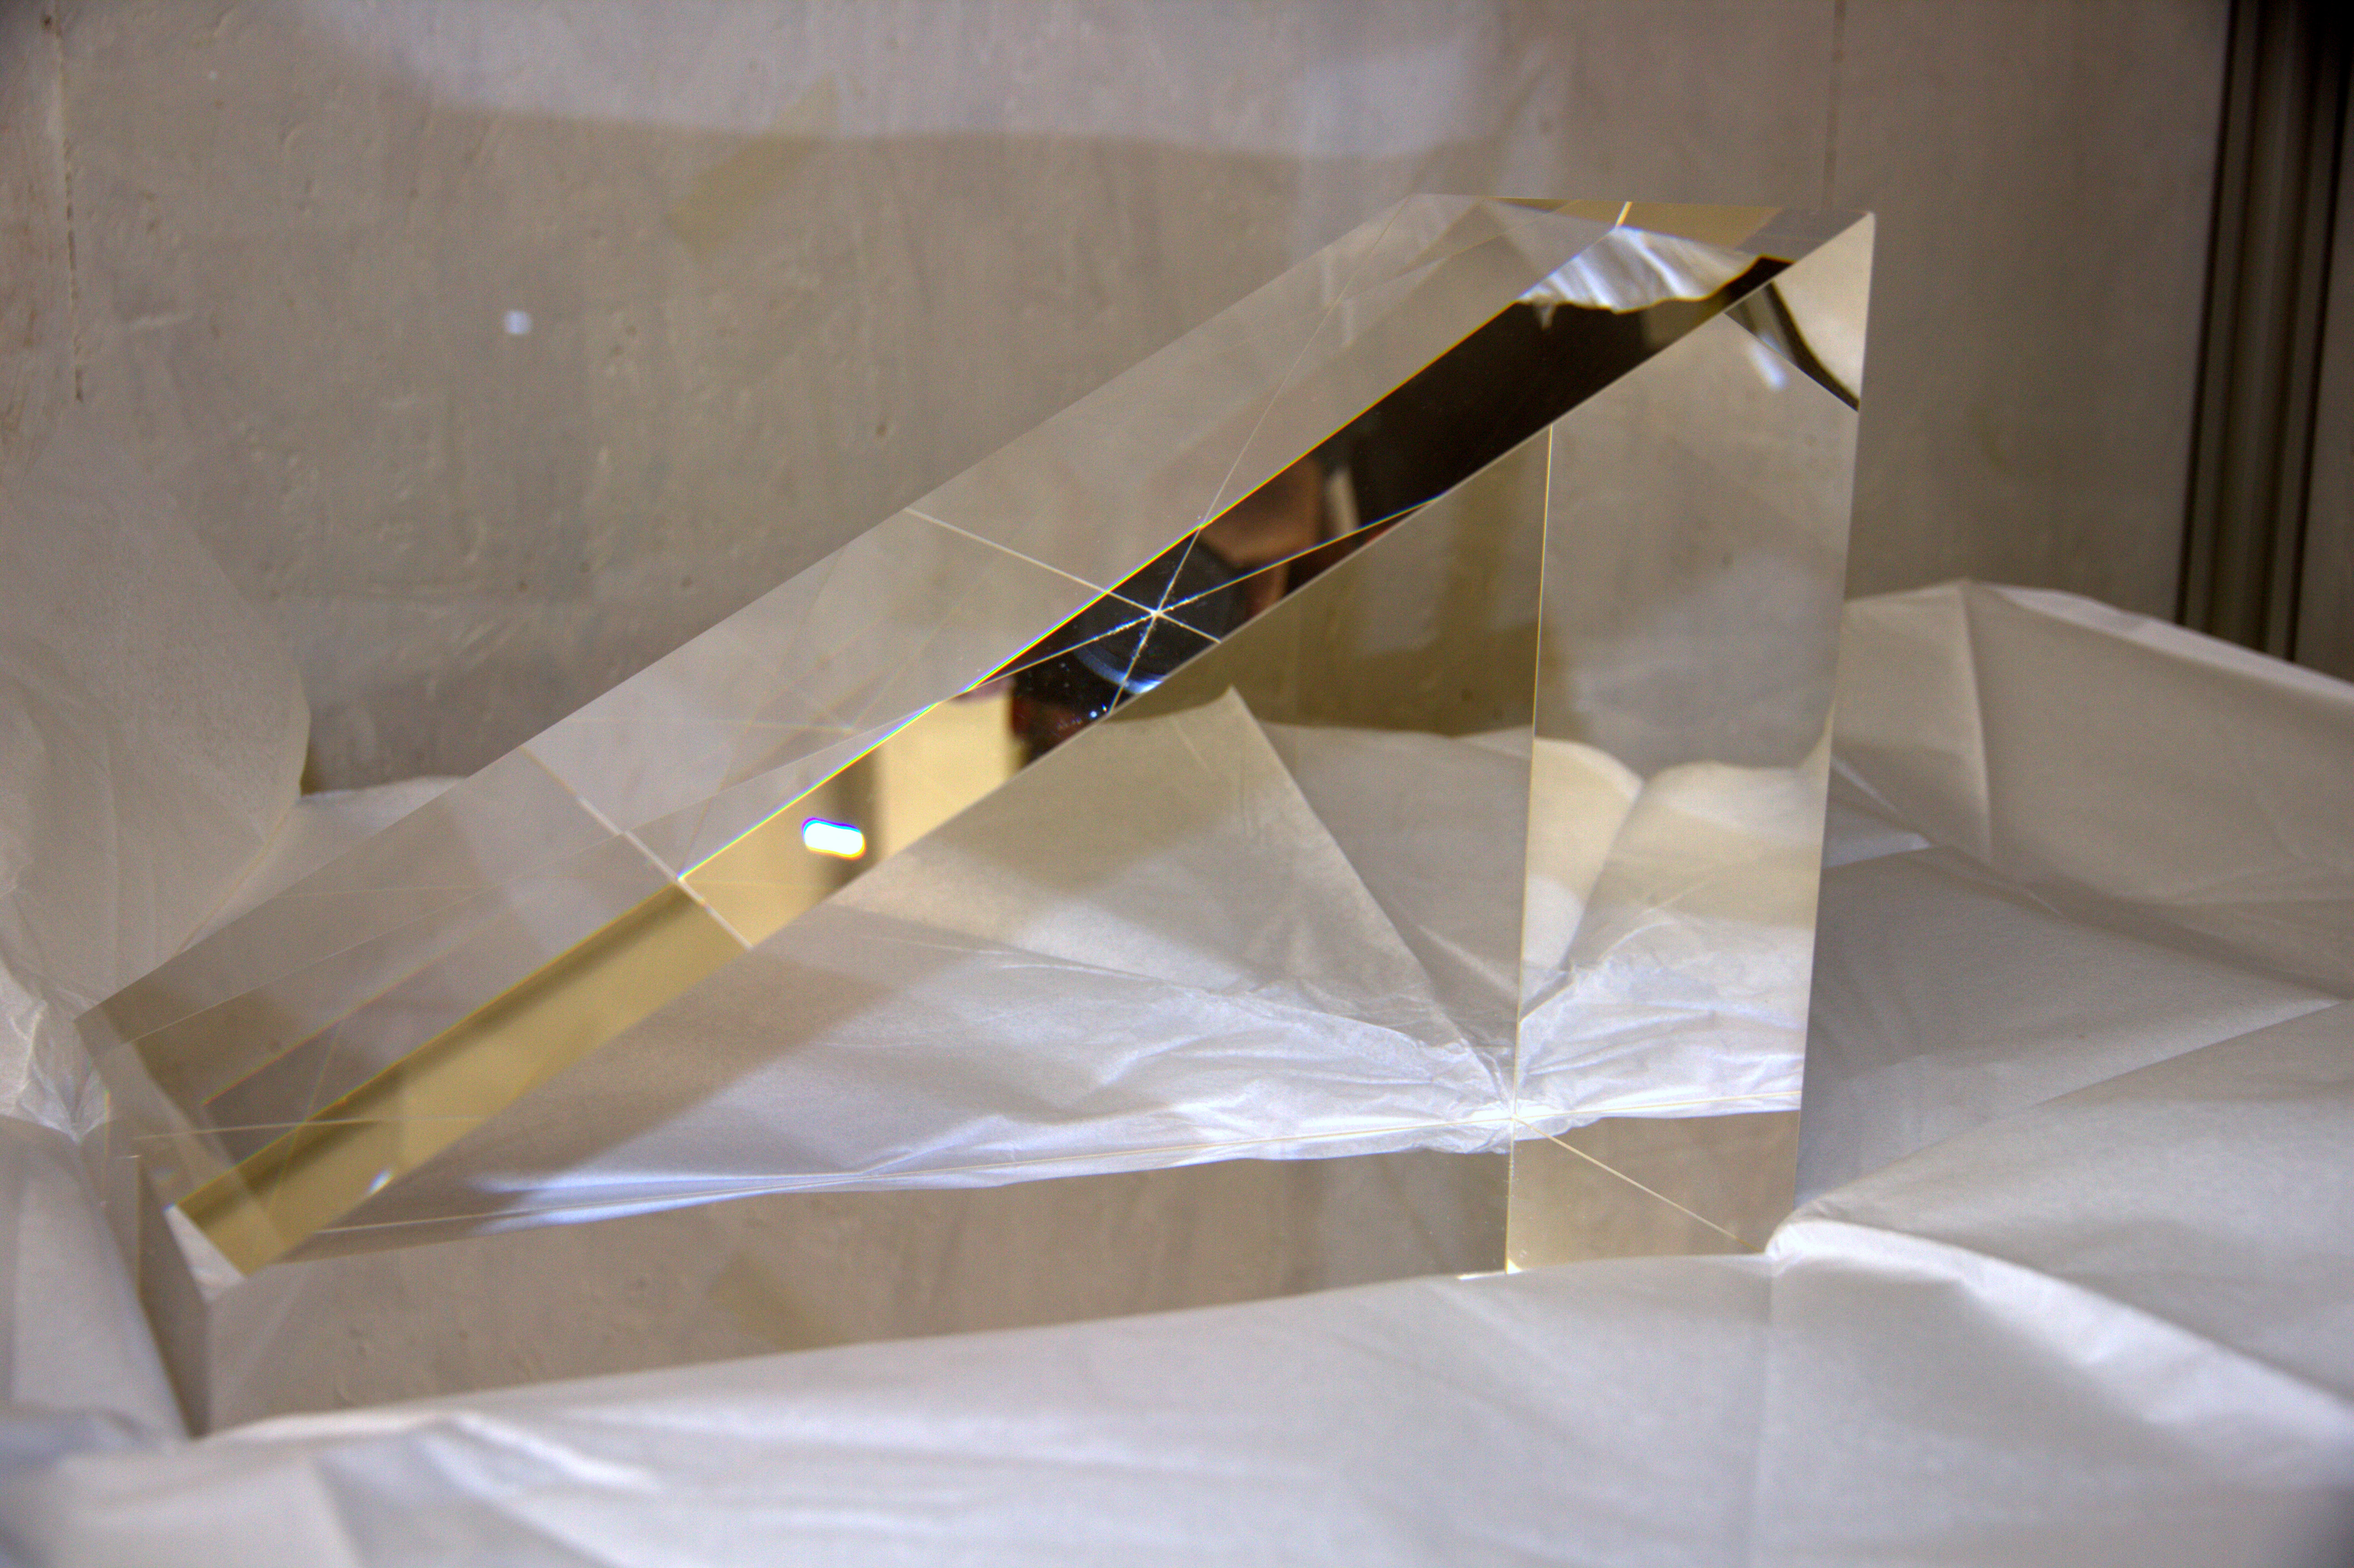
\includegraphics[width=0.7\textwidth]{30-deg-prism.pdf}
	\caption{Picture of the $30^{\circ}$ prism expansion volume used in the 2015 test beam.}
	\label{fig:prototype_prism}
\end{figure}

The optical component is attached to one end of the bar and a mirror is attached to the other. A compact prism expansion volume with dimensions $50\times170\times300\unit{mm}^3$ and an opening angle of $30^\circ$ (shown in Figure \ref{fig:prototype_prism}) was attached to the optical component (except in the case of an air-gap lens). A $3\times5$ array of PHOTONIS Planacon XP85102 MCP-PMTs with a total of 960 pixels ($6\times6\unit{mm}^2$ each) were held in place by a support structure and coupled to the expansion volume. The MCP-PMTs were read out by a DAQ system based on the trigger and readout board (TRB3) and the PADIWA discriminator card \cite{PANDA_electronics}. Couplings between the bar/lens, lens/prism, and prism/MCP-PMTs were done using Eljen EJ-550 optical grease \cite{EljenTech}. The mirror was not coupled directly to the bar, but held in place flat against the bar in order to prevent slight variations in grease thickness from effecting the angle of reflection.

The discriminating threshold signals for each MCP-PMT was adjusted and the difference between the discriminator and trigger signals were recorded by the TRB system. Noise events such as photons from delta electrons in the radiator bar and dark noise from the detectors were cut out using this timing information. Some channels had a very large background count rate and were masked. Calibration of the timing resolution of each channel was done using a 405 nm Picosecond Injection Laser (PiLas) PiL040SM by Advanced Laser Diode Systems \cite{PiLas} and a 660 nm Picosecond Pulsed Diode Laser (PDL 800-D) by PicoQuant \cite{PicoQuant}. The laser pulses were connected to an opal glass diffuser to illuminate the entire MCP-PMT plane. Calibrations were performed both daily and any time the geometric configuration was changed.

Data were taken for approximately 30 days, accumulating roughly 500 million triggers. Both bar and plate radiator geometries were tested with several optical components. Scans in polar angle between $20^\circ$ and $150^\circ$ were taken for many configurations. Scans in momentum up to 10 GeV/c were taken for select angles and geometries. As this was an opportunistic run for the EIC group, data taking was based on the needs of the PANDA DIRC group. They require separation power information for pion/kaon at 3.5 GeV/c, but since the T9 beam had a very small amount of kaons it was decided to instead study pion/proton separation at 7 GeV/c as the difference in Cherenkov angle for both cases is roughly 8 mrad. The results presented below will be from data taken with a bar radiator, 3-layer spherical lens, 7 GeV/c hadron-rich beam, and polar angles from  $20^\circ$ - $150^\circ$.

%----------------------------------------------------------------------
%	SIMULATION SECTION
%----------------------------------------------------------------------
\clearpage
\section{Prototype Simulation}
The accurate recreation of a DIRC detector in simulation is crucial for data analysis as it allows for the generation of the look-up-tables (LUTs) for geometric reconstruction, as well as a reference for the hit patterns \footnote{For the purposes of this document a ``hit" or ``photon" refers to a signal from a single pixel in an MCP-PMT. However because of an irreducible background it cannot be said for certain which signals are from true Cherenkov photons. What is truely measured are photo-electrons.} of the real-time monitoring system in the case of the 2015 CERN test beam campaign. A standalone GEANT4 simulation package was used for the CERN test beam, from which the EIC DIRC simulation in Chapter \ref{ch:eicdirc} was produced. Material properties for fused silica, NLaK33, the mirror, the optical grease, and the MCP-PMTs were included. The timing resolution of the simulation was based on findings of the laser calibration data and set to be 200 ps. For each configuration of the prototype the geometry for each element (e.g. relative positioning for the bar to the lens and prism) were adjusted to the values carefully measured while changing configurations.

\begin{figure}[!htb]
	\centering
	\includegraphics[width=\textwidth]{MCP_QE_2015.png}
	\includegraphics[width=\textwidth]{Photonis_QE.png}
	\caption{Channel-by-channel map of the relative quantum efficiency (QE) of each $6\times6\unit{mm}^2$ pixel of each MCP-PMT (64 pixels per MCP-PMT) used in the simulation of the 2015 test beam prototype (top). Absolute QE values in the simulation are the product of the channel-by-channel values with the wavelength dependent QE of a Planacon XP85012 MCP-PMT (bottom).}
	\label{fig:quantum_efficiency}
\end{figure}

Also included in the simulation is the quantum efficiency (QE) of the MCP-PMTs. Each MCP-PMT was scanned for QE and gain uniformity with a 372 nm laser pulser at Erlangen University. The mappings of QE were normalized to MCP-PMT 10 (when counting from bottom to top and left to right, starting at 0) and used as relative QE maps in the simulation (Figure \ref{fig:quantum_efficiency} top). To get the absolute QE for each pixel a scan was done of the QE as a function of photon wavelength (Figure \ref{fig:quantum_efficiency} bottom). The QE in the simulation was calculated by multiplying the relative QE of each pixel by the QE corresponding to the wavelength of the photon being detected by the pixel in the simulation.

\begin{figure}[!htb]
	\centering
	\includegraphics[width=0.7\textwidth]{proton_track_example.pdf}
	\caption{a) shows a visualization of the GEANT4 simulation of a single 7 GeV/c proton (red) traveling through the 2015 prototype with a bar radiator at a polar angle of $125^{\circ}$, b) is the accumulated hit pattern of 10,000 identical protons from simulation, and c) is the accumulated hit pattern of 10,000 tagged proton tracks from test beam data at 7 GeV/c beam and $125^{\circ}$ polar angle.}
	\label{fig:proton_track_example}
\end{figure}

Figure \ref{fig:proton_track_example}a shows an example of one simulated proton track with 7 GeV/c momentum (red) at a polar angle of $125^{\circ}$ traversing a bar radiator with the 3-layer lens focusing, and producing Cherenkov photons (yellow). Figure \ref{fig:proton_track_example}b is the accumulated hit pattern on the MCP-PMTs of 10,000 identical protons with the same configuration as in (a). Figure \ref{fig:proton_track_example}c is the accumulated hit pattern of 10,000 tagged proton events in the test beam data with 7 GeV/c beam momentum, $125^{\circ}$ polar angle, and the bar radiator and 3-layer lens configuration. The simulation very nicely reproduces the test beam hit pattern, giving a good indication that the simulation has the proper positioning of all the components.

%----------------------------------------------------------------------
%	DATA ANALYSIS SECTION
%----------------------------------------------------------------------
\clearpage
\section{Data Analysis}
Several studies were done during the CERN 2015 test beam campaign using both a radiator bar and plate, five different focusing configurations, and a range of momentum. Some studies were used as test runs for calibration and debugging. Information on the main data studies are shown in Table \ref{tab:runs2015}.

\begin{table}[]
\centering
\caption{Studies made during the 2015 CERN test beam campaign, including geometric configuration, momentum, and number of data points taken.}
\label{tab:runs2015}
\begin{tabular}{ccccc}
Study ID & Radiator & Lens & Momentum (GeV/c) & Data points \\
150 & bar & 2-layer spherical & 7 & 34 \\
151 & bar & 3-layer spherical & 7 & 46 \\
152 & plate & no lens & 7 & 28 \\
153 & plate & 2-layer cylindrical & 7 & 29 \\
154 & bar & 1-layer air gap & 7 & 44 \\
155 & bar & 1-layer air gap & 7 & 17 \\
157 & bar & 2-layer cylindrical & 7 & 43 \\
158 & bar & 3-layer spherical & 7 & 15 \\
159 & bar & no lens & 7 & 28 \\
160 & bar & 3-layer spherical & 5 & 47 \\
161 & plate & no lens & 5 & 29 \\
162 & plate & 2-layer cylindrical & 5 & 29 \\
170 & bar & 3-layer spherical & momentum scan & 9 \\
171 & plate & no lens & momentum scan & 8 \\
173 & plate & 2-layer cylindrical & momentum scan & 8 \\
174 & bar & 1-layer air gap & momentum scan & 8 \\
179 & bar & no lens & momentum scan & 9 \\
\end{tabular}
\end{table}


Two studies were chosen for the analysis in this thesis based on geometric configuration (bar and 3-layer lens) and momentum (7~GeV/c): 151 and 158. Study 151 is the primary data set because of its larger range in polar angle, while study 158 is used for comparison and error evaluation. Each data set represents approximately 1 day of beam.

\subsection{Event Selection}
The prototype data taken were stored in the list mode data format of the HADES DAQ system prototcol \cite{HADES_DAQ} and converted offline into the CERN ROOT data format \cite{ROOT} for analysis. The DAQ was started by a signal from Trigger 1, and events were required to have signals in Trigger 1, Trigger 2, and both TOF counters to ensure a well-defined beam spot and valid $\pi/p$ tagging from the TOF system. The veto counters were also required in event selection, but later found to be unnecessary for constraining the beam spot.

Hits were selected in a time window of $\pm 40$ ns relative to the Trigger 1 time. Channels with large electronics noise above 1 MHz and one defective PADIWA card were masked, with the same masking scheme applied to the simulation. Events with 5 or fewer MCP-PMT hits were also excluded from reconstruction due to lack of statistics for the reconstruction. It is also worth noting that, though the QE of the MCP-PMTs is more or less uniform, MCP-PMTs 12, 13, and 14 had poor performance during the test run due to electronics issues.

As mentioned previously the timing difference between the two TOF stations allowed for tagging an event as either pion or proton. Figure \ref{fig:tof_timing} shows the TOF time distributions for 5 GeV/c (top) and 7 GeV/c (bottom) beam momenta. These distributions were fitted with Gaussian functions near the proton and pion peaks and a $\pm2\sigma$ window around the peaks was used for selection (dashed lines).

\begin{figure}[!htb]
	\centering
	\includegraphics[width=\textwidth]{TOF_timing.pdf}
	\caption{Time difference between the two TOF stations for beam momenta of 5 GeV/c (top) and 7 GeV/c (bottom). The peaks were fitted and a $\pm2\sigma$ selection window was taken (dashed lines).}
	\label{fig:tof_timing}
\end{figure}

The timing of the hits in the MCP-PMTs were also constrained. Based on the orientation of the detector in the beam the time for the photon to propagate can be calculated based on the total bar path traveled ($Z$), using Figure \ref{fig:time_difference}a and
\begin{equation}
\begin{split}
	Z &= 
	\begin{cases}
		z_0 + \Delta z  & \text{direct photons} \\
		2L - z_0 - \Delta z  & \text{reflected photons}
	\end{cases}
	\\
	\Delta z &= -\cot(\alpha) \times \left[ D_2 + D_1\times\cot\left( 135 - \frac{\alpha}{2} \right) \right]
\end{split}
	\label{eq:time_diff_prop}
\end{equation}
%
where $L$ is the total length of the radiator, $z_0$ is the nominal perpendicular distance between the particle beam and the end of the radiator, $D_1$ is the distance from the pivot point of the radiator to the particle beam, $D_2$ is the distance from the pivot point to the radiator, and $\alpha$ is the polar angle.
Comparing the difference between the calculated expected arrival time and the actual arrival time of the photons gives a time difference distribution, shown in Figure \ref{fig:time_difference}b. In simulation it is to possible to exclude times associated with incorrect reconstructed paths from the LUT. Using this time distribution from only correct simulated paths it was determined that a time difference cut of $\pm1$~ns was sufficient across all polar angles for geometric reconstruction.

\begin{figure}[!htb]
	\centering
	\includegraphics[width=\textwidth]{time_difference.pdf}
	\caption{a) Illustration showing how total bar path length ($Z$) is calculated for the expected arrival time of photons based on distances from the pivot point (cyan circle) and particle beam ($D_1$),the pivot point to the radiator ($D_2$), nominal perpendicular distance between the beam and the end of the bar ($z_0$), and the polar angle ($\alpha$). Note that in the case of b) Example time difference distribution of experimental data (black), full simulation (red), and simulation including only correct prism paths from the LUT (blue) for $125^\circ$ polar angle. The dashed lines indicate the $\pm$1~ns cut taken during analysis. }
	\label{fig:time_difference}
\end{figure}


\subsection{Geometric Reconstruction}
The geometric reconstruction for the CERN 2015 test beam data was done in much the same manner as that described in Chapter \ref{ch:eicdirc}, however, three corrections were applied to the test beam data to improve resolution and overall performance: a correction to account for charge sharing between pixels in the MCP-PMTs, a per-MCP-PMT correction to the reconstructed mean $\thetaC$ for each polar angle, and a subtraction of the simulated path ambiguity background from beam data. Evaluation of the statistical and systematic uncertainties was also done for both simulation and beam data. Fitting of the main peak of the reconstructed Cherenkov angle was done in the same manner for both test beam data and simulation. Detailed information about the fitting for both protons and pions can be seen in Table \ref{tab:fitting_info} of Appendix \ref{appendix:fitting}. Results for photon yield, SPR, and reconstructed mean $\thetaC$ are presented below.

\subsubsection{Charge Sharing Correction}
It was discovered that many events in the prototype data showed multiple adjacent MCP-PMT pixels firing in a single event. It is difficult to say with certainty if neighboring firing pixels, such as the example shown in Figure \ref{fig:charge_sharing}a, fired independently or if charge sharing between the pixels occurred, effectively spreading the pixel's signal across multiple pixels. Because the width of each pixel corresponds to roughly a 20~mrad spread in Cherenkov angle the results of reconstructing these clustered pixels with the standard averaged LUT resulted in wider than expected reconstructed Cherenkov angle distributions for the prototype data. 

The solution was to modify the LUT to reconstruct the position of the photon not from the center of each pixel, but towards an edge, weighted by the position of neighboring firing pixels. Each pixel is subdivided into 9 sections in the LUT, as in Figure \ref{fig:charge_sharing}b. The reconstruction algorithm first determines if and where adjacent firing pixels are located for each hit and then reconstructs the Cherenkov angle at the center of the section most heavily weighted. Figure \ref{fig:charge_sharing_reco} shows the effect of this charge sharing correction for simulation (top) and experimental data (bottom) at $90^\circ$ polar angle. As was expected, the simulation, which does not include charge sharing, was largely unaffected. In the prototype data, however, the correction served to narrow the reconstructed Cherenkov angle peak and reduce background contributions.

\begin{figure}[!htb]
	\centering
	\includegraphics[width=\textwidth]{charge_sharing.pdf}
	\caption{a) A zoomed in view of a single MCP-PMT showing an example hit pattern from a single particle track. The 3 isolated pixels (red) have no neighboring hits. The 3 clustered hits (green), however, are adjacent to other firing pixels and thus it is hard to determine with timing alone if these are the result of a single photon from the bottom right pixel that resulted in charge sharing, 3 independent photons hitting all 3 pixels, or some combination of 2 photons hitting 2 of the pixels that resulted in charge sharing. To compensate for this uncertainty each pixel is subdivided, as in (b), into 9 regions such that the LUT will reconstruct the photon angle from different areas of the pixel. For the case of (a) the top pixel in the cluster would be reconstructed from point 7, the bottom left pixel from point 5, and the bottom right pixel from point 2, while the 3 isolated pixels would all be reconstructed from point 0.}
	\label{fig:charge_sharing}
\end{figure}

\begin{figure}[!htb]
	\centering
	\includegraphics[width=\textwidth]{chargeshare_90_sim.png}
	\includegraphics[width=\textwidth]{chargeshare_90_data.png}
	\caption{Reconstructed Cherenkov angle of 7 GeV/c protons for simulation (top) and prototype data (bottom) for $90^\circ$ polar angle using the standard LUT (blue) and the charge-sharing-corrected LUT (red). The simulation is largely unaffected, while in the data the peak has been narrowed and the background reduced.}
	\label{fig:charge_sharing_reco}
\end{figure}


\subsubsection{Per-MCP-PMT $\theta_{C}$ Correction}
The fitted mean of the reconstructed Cherenkov angle from geometric reconstruction showed a non-constant value across the prototype polar angle range for both simulation and experimental data. To correct for this non-constant shift a per-MCP-PMT $\thetaC$ correction was implemented in the reconstruction. For a given polar angle and particle species the reconstructed Cherenkov angle for each MCP-PMT is fitted in the same manner as the full data set and a value for the Cherenkov angle is extracted (see Figure \ref{fig:mcp_corr_hist}). The difference between the extracted value and the true value define a shift that is then used to adjust the Cherenkov angle spectrum for each individual MCP-PMT. After corrections the mean Cherenkov angle is much more accurately reproduced, and even improves the SPR at the some polar angles. Figure \ref{fig:mcp_corr_polar} shows the results of the correction for the full range of polar angles.

\begin{figure}[!htb]
	\centering
	\includegraphics[width=\textwidth]{mcp_shift_hist.png}
	\caption{Reconstructed $\thetaC$ at $90^\circ$ polar angle before (red) and after (blue) per-MCP-PMT corrections. The uncorrected distribution has an SPR (the $\sigma$ of the gaussian) of 10.9~mrad and a mean $\thetaC$ of 823.1~mrad, or 6.3~mrad away from the true value of 816.8~mrad for a 7~GeV/c proton. The corrected distribution has a steady SPR of 10.9~mrad and a mean of 813.4~mrad, which is only 3.4~mrad away from the true value.}
	\label{fig:mcp_corr_hist}
\end{figure}


\begin{figure}[!htb]
	\centering
	\includegraphics[width=\textwidth]{mcp_corr_polar.pdf}
	\caption{\textbf{Top}: Reconstructed mean $\thetaC$ before applying per-MCP-PMT corrections for simulation (blue) and prototype data (red) for 7 GeV/c protons. The dashed line indicates the true Cherenkov angle for a 7 GeV/c proton of 816 mrad. \textbf{Bottom}: Reconstructed $\thetaC$ after applying corrections.}
	\label{fig:mcp_corr_polar}
\end{figure}


\subsubsection{Simulated Background Subtraction}
Because the majority of the background signal for the reconstructed Cherenkov angle comes from irreducible photon path ambiguities it would stand to reason that the ambiguity background simulated in GEANT4 would reasonably describe the PANDA prototype background seen in the experimental data, assuming the geometry has been correctly recreated in GEANT4. Figure \ref{fig:background_sub}a shows a simulation of 1000 protons at 7 GeV/c and $125^\circ$ polar angle along with the ambiguity background (i.e. the reconstructed Cherenkov angle coming from incorrect prism ambiguities) and the reconstructed angles coming from true prism paths. Figure \ref{fig:background_sub}b shows the prototype data with the same configuration along with the simulated background and the background-subtracted data. Because of the nice description of the background from simulation, the background-subtracted prototype data shows a clear peak and minimal background. This method could prove to be very useful for and EIC DIRC as the already minimal geometric background (see Figure \ref{fig:EIC_reconstruction} as an example) could be nearly eliminated.

\begin{figure}[!htb]
	\centering
	\includegraphics[width=\textwidth]{background_subtraction.pdf}
	\caption{(a) The full reconstructed Cherenkov angle (blue line), reconstructed angle with only incorrect prism path ambiguities (black circles), and the reconstructed angle assuming only true prism paths (red histogram) for $125^\circ$ polar angle protons from simulation. (b) Beam data (blue line) with path ambiguity background from simulation (black circles, same as (a)). The red histogram is the difference between blue and black.}
	\label{fig:background_sub}
\end{figure}

\subsubsection{Evaluation of Uncertainties}
Many factors were considered for both the statistical and systematic uncertainties associated with the geometric reconstruction method: internal file consistency \footnote{Taking 100 sets of 100 events and running the reconstruction analysis for each set as normal.}, varying the fitting function and fit range found to be optimal for each polar angle, varying histogram binning, varying the timing cuts, and checking the stability of a given geometric configuration between studies 151 and 158. For each contribution to the error, multiple samples were taken and the RMS of the distribution for photon yield (where applicable), SPR, and mean $\thetaC$ were taken to be the associated error. Derived errors for tagged protons in both experimental data and simulation are shown in Tables \ref{tab:err_data} and \ref{tab:err_sim} of Appendix \ref{appendix:error} respectively.

Select polar angles were reconstructed for both studies 151 and 158 and compared (see Figures \ref{fig:compare_158_NPH}, \ref{fig:compare_158_SPR}, and \ref{fig:compare_158_THC}). The difference in photon yield, SPR, and mean $\thetaC$ were all found to be very small compared to the contributions coming from other systematics (thus confirming that the CERN setup was very stable) and were not included in the final error bars, but are shown in Table \ref{tab:err_data} for completeness.

\begin{figure}[!htb]
	\centering
	\includegraphics[width=\textwidth]{compare_158_NPH.pdf}
	\caption{Comparison of the extracted photon yield of studies 151 (red) and 158 (green). All common polar angles agree nicely.}
	\label{fig:compare_158_NPH}
\end{figure}

\begin{figure}[!htb]
	\centering
	\includegraphics[width=\textwidth]{compare_158_SPR.pdf}
	\caption{Comparison of the extracted SPR of studies 151 (red) and 158 (green). All common polar angles other than $50^\circ$ agree.}
	\label{fig:compare_158_SPR}
\end{figure}

\begin{figure}[!htb]
	\centering
	\includegraphics[width=\textwidth]{compare_158_THC.pdf}
	\caption{Comparison of the reconstructed mean $\thetaC$ of studies 151 (red) and 158 (green). All common polar angles other than $50^\circ$ agree.}
	\label{fig:compare_158_THC}
\end{figure}

\subsubsection{Results}
Figure \ref{fig:2015_NPH} shows the extracted photon yield for the CERN 2015 test beam data. The enhancement of the photon yield at 90 degrees for simulation compared to beam data can be understood by recalling that the MCP-PMTs at the base of the expansion volume (12, 13, and 14) had poor performance during the test beam and these sensors are where nearly 100\% of the produced Cherenkov photons end up from a $90^\circ$ polar angle track.

Figures \ref{fig:2015_THC_nocorr}, \ref{fig:2015_THC_bg_nocorr}, \ref{fig:2015_THC_mcpcorr}, and \ref{fig:2015_THC_bg_mcpcorr} show the final results for the reconstructed mean $\thetaC$ of the CERN 2015 beam data and simulation for protons and pions both with and without per-MCP-PMT corrections and path ambiguity background subtraction. As per the design, the per-MCP-PMT correction gives a much cleaner separation between protons and pions while also shifting the simulation and beam data such that they are in good agreement both with each other and with the expected Cherenkov angle. The path ambiguity background subtraction, however, does not significantly improve the performance of the reconstructed $\thetaC$ in either case. This is to be expected in both cases as the distribution of the background under the simulated peak is typically flat. It should, however, show some improvement for the SPR.

Figures \ref{fig:2015_SPR_prot_nocorr}, \ref{fig:2015_SPR_prot_mcpcorr}, \ref{fig:2015_SPR_prot_bg_nocorr}, \ref{fig:2015_SPR_prot_bg_mcpcorr}, \ref{fig:2015_SPR_pion_nocorr}, \ref{fig:2015_SPR_pion_mcpcorr}, \ref{fig:2015_SPR_pion_bg_nocorr}, and \ref{fig:2015_SPR_pion_bg_mcpcorr} show the final results for the SPR of the CERN 2015 beam data and simulation for protons and pions both with and without per-MCP-PMT corrections and path ambiguity background subtraction. Unlike the reconstructed Cherenkov angle, here the per-MCP-PMT correction has little effect on the extraction of the SPR. This result is somewhat counterintuitive as one would expect that shifting each MCP-PMT's $\thetaC$ spectrum separately to the correct value would naturally narrow the signal peak. This, however, does not seem to be the case for most polar angles. Utilizing the path ambiguity background subtraction, on the other hand, shows a significant improvement of the SPR for most polar angles. Overall the beam data and GEANT4 simulation are in fairly good agreement for most polar angles, and within an acceptable value for PID performance.

Figure \ref{fig:2015_LUT_separation} shows the proton/pion log-likelihood separation for both simulation and beam data for geometric reconstruction. The simulated separation power meets the $3\sigma$ performance expected by the PANDA DIRC group for a majority of the polar angle range. However, the beam data shows a much worse performance, dropping to around $1\sigma$ for near perpendicular angles. This can most 

Figure \ref{fig:2015_LUT_efficiency} shows the PID and misidentification (MisID) probability for protons (e.g. the MisID for protons shows the probability of a proton to be misidentified as a pion) as a function of polar angle for geometric reconstruction. MisID is calculated by taking the integral of the Gaussian fit from the crossing of the two curves (shown with the red circle) out to the tail of the distribution and dividing by the total integral of the curve. The PID probability is then 1-MisID.

%===========NPH==============%
\begin{figure}[!htb]
	\centering
	\includegraphics[width=\textwidth]{2015_NPH.pdf}
	\caption{Extracted photon yield from GEANT4 simulation (blue) and study 151 of the 2015 CERN test beam data.}
	\label{fig:2015_NPH}
\end{figure}

%===========THC==============%
\begin{figure}[!htb]
	\centering
	\includegraphics[width=\textwidth]{2015_THC_nocorr.pdf}
	\caption{Reconstructed mean $\thetaC$ with no background subtraction and no per-MCP-PMT correction from GEANT4 simulation (blue) and study 151 of the 2015 CERN test beam data (red) for protons (filled circles) and pions (open circles). The solid and dashed lines indicate the true Cherenkov angle for 7 GeV/c pions and protons respectively.}
	\label{fig:2015_THC_nocorr}
\end{figure}

\begin{figure}[!htb]
	\centering
	\includegraphics[width=\textwidth]{2015_THC_bg_nocorr.pdf}
	\caption{Reconstructed mean $\thetaC$ with simulated background subtraction but no per-MCP-PMT correction from GEANT4 simulation (blue) and study 151 of the 2015 CERN test beam data (red) for protons (filled circles) and pions (open circles). The solid and dashed lines indicate the true Cherenkov angle for 7 GeV/c pions and protons respectively.}
	\label{fig:2015_THC_bg_nocorr}
\end{figure}

\begin{figure}[!htb]
	\centering
	\includegraphics[width=\textwidth]{2015_THC_mcpcorr.pdf}
	\caption{Reconstructed mean $\thetaC$ with no background subtraction but using a per-MCP-PMT correction from GEANT4 simulation (blue) and study 151 of the 2015 CERN test beam data (red) for protons (filled circles) and pions (open circles). The solid and dashed lines indicate the true Cherenkov angle for 7 GeV/c pions and protons respectively.}
	\label{fig:2015_THC_mcpcorr}
\end{figure}

\begin{figure}[!htb]
	\centering
	\includegraphics[width=\textwidth]{2015_THC_bg_mcpcorr.pdf}
	\caption{Reconstructed mean $\thetaC$ with simulated background subtraction and using a per-MCP-PMT correction from GEANT4 simulation (blue) and study 151 of the 2015 CERN test beam data (red) for protons (filled circles) and pions (open circles). The solid and dashed lines indicate the true Cherenkov angle for 7 GeV/c pions and protons respectively.}
	\label{fig:2015_THC_bg_mcpcorr}
\end{figure}

%===========SPR PROTONS==============%
\begin{figure}[!htb]
	\centering
	\includegraphics[width=\textwidth]{2015_SPR_prot_nocorr.pdf}
	\caption{Fitted SPR for proton-tagged events of study 151 of the CERN 2015 test beam data (red) and GEANT4 simulation (blue) without background subtraction or a per-MCP-PMT correction.}
	\label{fig:2015_SPR_prot_nocorr}
\end{figure}

\begin{figure}[!htb]
	\centering
	\includegraphics[width=\textwidth]{2015_SPR_prot_mcpcorr.pdf}
	\caption{Fitted SPR for proton-tagged events of study 151 of the CERN 2015 test beam data (red) and GEANT4 simulation (blue) without background subtraction and using a per-MCP-PMT correction.}
	\label{fig:2015_SPR_prot_mcpcorr}
\end{figure}

\begin{figure}[!htb]
	\centering
	\includegraphics[width=\textwidth]{2015_SPR_prot_bg_nocorr.pdf}
	\caption{Fitted SPR for proton-tagged events of study 151 of the CERN 2015 test beam data (red) and GEANT4 simulation (blue) using simulated background subtraction but no per-MCP-PMT correction.}
	\label{fig:2015_SPR_prot_bg_nocorr}
\end{figure}

\begin{figure}[!htb]
	\centering
	\includegraphics[width=\textwidth]{2015_SPR_prot_bg_mcpcorr.pdf}
	\caption{Fitted SPR for proton-tagged events of study 151 of the CERN 2015 test beam data (red) and GEANT4 simulation (blue) using both simulated background subtraction and a per-MCP-PMT correction.}
	\label{fig:2015_SPR_prot_bg_mcpcorr}
\end{figure}

%===========SPR PIONS==============%
\begin{figure}[!htb]
	\centering
	\includegraphics[width=\textwidth]{2015_SPR_pion_nocorr.pdf}
	\caption{Fitted SPR for pion-tagged events of study 151 of the CERN 2015 test beam data (red) and GEANT4 simulation (blue) without background subtraction or a per-MCP-PMT correction.}
	\label{fig:2015_SPR_pion_nocorr}
\end{figure}

\begin{figure}[!htb]
	\centering
	\includegraphics[width=\textwidth]{2015_SPR_pion_mcpcorr.pdf}
	\caption{Fitted SPR for pion-tagged events of study 151 of the CERN 2015 test beam data (red) and GEANT4 simulation (blue) without background subtraction and using a per-MCP-PMT correction.}
	\label{fig:2015_SPR_pion_mcpcorr}
\end{figure}

\begin{figure}[!htb]
	\centering
	\includegraphics[width=\textwidth]{2015_SPR_pion_bg_nocorr.pdf}
	\caption{Fitted SPR for pion-tagged events of study 151 of the CERN 2015 test beam data (red) and GEANT4 simulation (blue) using simulated background subtraction but no per-MCP-PMT correction.}
	\label{fig:2015_SPR_pion_bg_nocorr}
\end{figure}

\begin{figure}[!htb]
	\centering
	\includegraphics[width=\textwidth]{2015_SPR_pion_bg_mcpcorr.pdf}
	\caption{Fitted SPR for pion-tagged events of study 151 of the CERN 2015 test beam data (red) and GEANT4 simulation (blue) using both simulated background subtraction and a per-MCP-PMT correction.}
	\label{fig:2015_SPR_pion_bg_mcpcorr}
\end{figure}

%===========LOG SEPARATION==============%
\begin{figure}[!htb]
	\centering
	\includegraphics[width=\textwidth]{2015_LUT_separation.pdf}
	\caption{Proton/pion log-likelihood separation using geometric reconstruction for simulation (blue) and beam data (red) using a 3-layer lens, radiator bar, and 7 GeV/c beam momentum.}
	\label{fig:2015_LUT_separation}
\end{figure}

%===========PID==============%
\begin{figure}[!htb]
	\centering
	\includegraphics[width=\textwidth]{2015_LUT_efficiency.pdf}
	\caption{PID (closed circles) and MisID (open circles) probabilities for simulated protons (blue) and tagged proton events in beam data (red). Results for pions are similar for both simulation and beam data.}
	\label{fig:2015_LUT_efficiency}
\end{figure}

\clearpage
\subsection{Time-based Reconstruction}
The time-based reconstruction of the 2015 CERN data was done in the same manner as the time-based reconstruction of the EIC simulation described in Chapter \ref{ch:eicdirc}. PDFs for the beam data were created by using every other event in a data file for both pions and protons. The reconstruction of the data was done with the other half of the data file to ensure no ``cross talk" was occurring that would give an inaccurate result. Figure \ref{fig:2015_timebased_example} shows the log-likelihood separation for $90^\circ$ and $25^\circ$ polar angles along with the separation power, given in unites of standard deviations (std dev) and calculated by dividing the distance between the two peaks of the distributions by their average standard deviations.

\begin{figure}[!htb]
	\centering
	\includegraphics[width=\textwidth]{2015_timebased_example.pdf}
	\caption{Log-likelihood separation for $90^\circ$ (left) and $25^\circ$ (right) polar angles for pions (blue) and protons (red). Particles identified as protons will tend towards the right side of the zero point, while particles identified as pions will tend towards the left side of the zero point. The calculated separation power for each distribution are 1.48 and 3.5 standard deviations (std dev) respectively.  The overlap of one curve under another will give the misidentification (MisID) of that species as being identified as the other.}
	\label{fig:2015_timebased_example}
\end{figure}

\subsubsection{Results}
\begin{figure}[!htb]
	\centering
	\includegraphics[width=\textwidth]{2015_timebased_separation.pdf}
	\caption{Proton/pion log-likelihood separation using time-based imaging for simulation (blue) and beam data (red) using 3-layer lens, radiator bar, and 7 GeV/c beam momentum.}
	\label{fig:2015_timebased_separation}
\end{figure}

Figure \ref{fig:2015_timebased_separation} shows the separation power for the radiator bar with the 3-layer lens and 7 GeV/c beam momentum as a function of polar angle for simulation and beam data. Clearly the beam data was not able to reach the desired $3\sigma$ separation. This is caused in part by the timing resolution, which for the prototype was a factor of 2-3 worse than expected. Another factor contributing to the discrepancy is the photon detection efficiency loss of the lower quality MCP-PMTs at the base of the expansion volume, as is evident by the lack of a rise in the separation power near $90^\circ$ polar angle in the beam data compared to simulation.

\begin{figure}[!htb]
	\centering
	\includegraphics[width=\textwidth]{2015_timebased_efficiency.pdf}
	\caption{PID (closed circles) and MisID (open circles) probabilities for simulated protons (blue) and tagged proton events in beam data (red). Results for pions are similar for both simulation and beam data.}
	\label{fig:2015_timebased_efficiency}
\end{figure}
Figure \ref{fig:2015_timebased_efficiency} shows the PID and MisID probability for protons as a function of polar angle Results for pion PID and MisID probability are similar to that of the proton. Again, due to the worse timing resolution than expected, the MisID is much worse for the beam data than the simulation.
